	\section{\textbf{Magnetómetro}} Un magnetómetro es un instrumento pasivo que mide las variaciones en el campo magnético terrestre. En la exploración oceánica, se utiliza para identificar sitios de patrimonio cultural, como restos de naufragios de barcos y aviones, así como para caracterizar formaciones geológicas en el fondo marino.

\subsection{\textbf{¿Cómo Funciona un Magnetómetro?}}
El magnetómetro opera midiendo las variaciones en el campo magnético terrestre mediante distintos principios de detección. Su funcionamiento se basa en la detección de fuerzas magnéticas generadas por materiales ferromagnéticos, permitiendo identificar objetos y anomalías en el entorno.  

\subsubsection{\textbf{Principio de Funcionamiento}}
\begin{itemize}
	\item El núcleo terrestre genera un campo magnético debido a la circulación de metales líquidos en su interior.
	\item Cuando un magnetómetro se desplaza, registra las variaciones en la intensidad magnética.
	\item Al detectar objetos metálicos, el sensor capta anomalías magnéticas y las representa en un gráfico de datos.
\end{itemize}

\subsection{\textbf{Tipos de Magnetómetros}}
Existen distintos tipos de magnetómetros según su método de detección:
\begin{itemize}
	\item \textbf{Magnetómetros de Protones}: Miden la frecuencia de precesión de protones en un campo magnético.
	\item \textbf{Magnetómetros de Efecto Hall}: Detectan cambios de voltaje en respuesta a campos magnéticos.
	\item \textbf{Magnetómetros SQUID}: Utilizan superconductores para detectar variaciones magnéticas extremadamente pequeñas.
\end{itemize}
\subsection{\textbf{¿Para qué Sirve un Magnetómetro?}}
El magnetómetro tiene diversas aplicaciones en múltiples campos, entre ellas:

\subsubsection{\textbf{Exploración Oceánica y Arqueología Submarina}}
\begin{itemize}
	\item Detecta naufragios, anclas y artefactos metálicos sumergidos.
	\item Identifica estructuras enterradas en el lecho marino sin necesidad de excavación.
\end{itemize}

\subsubsection{\textbf{Geofísica y Exploración Geológica}}
\begin{itemize}
	\item Permite localizar depósitos minerales, como magnetita y hematita.
	\item Ayuda en la detección de fallas geológicas y estructuras volcánicas.
\end{itemize}

\subsubsection{\textbf{Navegación y Orientación}}
\begin{itemize}
	\item Se emplea en sistemas de navegación de submarinos y aeronaves.
	\item Integrado en dispositivos electrónicos como teléfonos móviles y drones para determinar la dirección magnética.
\end{itemize}

\subsubsection{\textbf{Seguridad y Defensa}}
\begin{itemize}
	\item Se usa para detectar submarinos y minas marinas en operaciones militares.
	\item Aplicado en aeropuertos y controles de seguridad para identificar objetos metálicos ocultos.
\end{itemize}

\subsubsection{\textbf{Investigación Astronómica y Espacial}}
\begin{itemize}
	\item Permite el estudio del campo magnético de planetas y lunas.
	\item Se utiliza en misiones espaciales para medir la magnetosfera terrestre y detectar anomalías magnéticas en otros cuerpos celestes.
\end{itemize}
\begin{figure}[H]
	\centering
	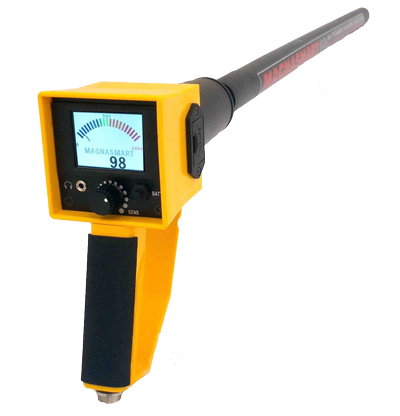
\includegraphics[width=0.3\textwidth]{magnetometro.png}
	\caption{Magnetómetro}
\end{figure}
